\documentclass[11pt,a4paper]{article}
% \renewcommand\normalsize{\fontsize{12}{18.0pt}\selectfont}
\usepackage[utf8]{inputenc}
\usepackage[T2A]{fontenc}
\usepackage[russian]{babel}
\usepackage{graphicx}
\usepackage{amsmath,amssymb,amsthm}
\usepackage{epsfig}
\usepackage{import}
\usepackage{wrapfig}
\usepackage{epigraph}
\usepackage{verbatim}
\usepackage{soul}
\usepackage[usenames]{color}
\usepackage{listings}
\usepackage{pdfpages}

\usepackage[pdf]{graphviz}


\pagestyle{empty}

\hoffset=-15mm    %по горизонтали влево на \hoffset
\voffset=-37.5mm  %по вертикали вверх на \voffset
\textheight=275mm
\textwidth=155mm


\newcommand{\eps}{\varepsilon}
\renewcommand{\phi}{\varphi}
\newcommand{\Impl}{\ensuremath{\Rightarrow}}
\newcommand{\RRR}{\overline{\mathbb{R}}}
\newcommand{\RR}{\mathbb{R}}
\newcommand{\NN}{\mathbb{N}}
\newcommand{\QQ}{\mathbb{Q}}
\newcommand{\nl}{\newline}

\usepackage{ifthen}
\newcommand\ifnonempty[2]{\ifthenelse{\equal{#1}{}}{}{#2}}
% Команда \task для условий задач с одним необязательным аргументом
% \defin определения, \exerc упражнения \prop предложения \theor теорема
\newcounter{task}
\newcounter{defin}
\newcounter{prop}
\newcounter{thm}
\newcounter{lem}
\newcommand{\task}[1][]{\smallskip\par\hangafter=1\normalsize\textbf{Задача \refstepcounter{task}\thetask\ifnonempty{#1}{ (#1)}.}~}
\newcommand{\defin}[1][]{\smallskip\par\hangafter=1\normalsize\textbf{Определение \refstepcounter{defin}\thedefin\ifnonempty{#1}{ (#1)}.}~}
\newcommand{\exerc}[1][]{\smallskip\par\hangafter=1\normalsize\textbf{Упражнение \refstepcounter{task}\thetask\ifnonempty{#1}{ (#1)}.}~}
\newcommand{\prop}[1][]{\smallskip\par\hangafter=1\normalsize\textbf{Предложение \refstepcounter{prop}\theprop\ifnonempty{#1}{ (#1)}.}~}
\newcommand{\thm}[1][]{\smallskip\par\hangafter=1\normalsize\textbf{Теорема \refstepcounter{thm}\thethm\ifnonempty{#1}{ (#1)}.}~}
\newcommand{\lem}[1][]{\smallskip\par\hangafter=1\normalsize\textbf{Лемма \refstepcounter{lem}\thelem\ifnonempty{#1}{ (#1)}.}~}
% \setcounter{thm}{2}

\begin{document}
\begin{center}
\Huge {
\noindent
\textbf{Задача о минимальной надстроке}
}
\end{center}
\begin{center}
Жуков Владислав 499
\end{center}
В данной работе рассматривается задача о минимальной надстроке. Доказывается ее $NP$ полнота, а также рассматриваются приближенные алгоритмы для ее решения.
\\Дадим формальное определение для этой задачи, а также понятиям, которые нам понадобятся при доказательстве ее $NP$ полноты
\defin
Пусть задано множество строк $A = \alpha_1, \alpha_2, ..., \alpha_n$ над конечным алфавитом. Требуется найти такую строку $\omega$, что
все строки из множества $A$ являются подстроками $\omega$ и длина $\omega$ минимальна. Назовем эту задачу "задачей о надстроке" или SSP.
\defin
$overlap(s_1, s_2)$ Это длина наибольшего x, такого что $s_1 = ax$ и $s_2 = xb$ для некоторых строк $a$ и $b$. Проще говоря, это длина максимально возможного перекрытия двух строк.
\defin
$pr(s1, s2)$ Это строка $a$ из предыдущего определения.
\\
Понятно, что длина минимальной надстроки для двух строк - это длина строки, получившейся путем "схлапывания"(т.е. конкатинации с удалением перекрытия $x$ из определения) двух строк в правильном порядке.
(для строк $a$ и $b$ длина их надстроки будет: $|a| + |b| - overlap(a, b)$). Вообще говоря, для любого количества строк, надстрока для них получается путем схлапывания этих строк в некотором правильном порядке.
На этой простой идее будут основываться все приблеженные алгоримы во второй части работы.
\\ Доказывать $NP$ полноту будем, сводя задачу о Гамильтоновом пути к нашей задаче. Поэтому нам понадобятся следующие определения.
\defin $G(V, E)$ обозначает граф $G$ с множеством вершин $V$ и множеством ребер $E$.
\defin Для неориентированного графа $IN(v), OUT(v)$ - обозначают количество входящих и выходящих ребер соответственно из вершины v.
\defin $\oplus$ обозначает сложение по модулю $OUT(v)$ для вершины $v$(вершина будет указана явно).
\defin (Задача об ограниченном направленном Гамильтоновом пути)
\\
\textit{Задача напревленного Гамильтонова пути:}
\par Дан ориентированный граф $G$, есть ли в нем путь проходящий по всем вершинам ровно по одному разу.  Про эту задачу известно, что он NP-полная.
\\
\textit{Задача ограниченного направленного Гамильтонова пути:}
\parЭто задача направленного Гамильтонова пути сго следующими ограничениями:
\\Есть назначенная стартовая вершина $s$ и конечная вершина $t$, такие, что $IN(s) = OUT(t) = 0$. Все вершины кроме конечной вершины $t$, имеют исходящую степень большую 1.
\\ Идея доказательства $NP$ полноты состоит в том, чтобы построить по данному нам графу такое множество строк, что минимальная надстрока задавала бы гамильтонов путь в этом графе, таким образом мы сведем
задачу ограниченного направленного Гамильтонова пути к задаче о минимальной надстроке.
\thm
SSP с бесконечным алфавитом является  NP-полной.
%Более того, это задача NP-полна даже если для любого $H \ge 3$, при ограничении на то, что все строки примитивные длины H
\par
\textit{Доказательство:}
% Для начала докажем для неприметивных строк длины 3, а после покажем как изменить конструкцию, чтобы сделать все строки примитивными длины H, для $H \ge 3$.
Пусть $G = (V, E)$ это граф из задачи ограниченного напревленного Гамильтонова пути, где $V$ это множество целых чисел от 1 до n(1 это начальная вершина и n это конечная вершина) и $|E| = m$.
Мы построим строки для $G$ над алфавитом $\Sigma = V \cup B \cup S$, где $B = \{\overline{v}| v \in V - \{n\} \}$ множество "запрещенных" символов, а S - множество специальных символов.
Запрещенные символы являются "локальными" для каждой вершины, тогда как специальные являются "глобальными" символами для всего графа $G$.
Для каждой вершины $v \in V - \{v\}$ мы сопоставим множество $A_v$ содержащее $2OUT(v)$ строк. Пусть $R_v = \{\omega_0, ..., \omega_{OUT(v) - 1}\}$ это множество вершин соединенных с $v$.
Тогда, $A_v = \{\overline{v}\omega_i\overline{v}|\omega_i \in R_v\} \cup \{\omega_i \overline{v}\omega_{i \oplus 1}| \omega_i \in R_v\}$, где $\oplus$ обозначает сложение по модулю $OUT(v)$.
\par
Для каждой вершины $v \in V - \{1, n\}$ создаем множество $C_v$ из одного элемента, содержащее строку $v \# \overline{v}$ называемую соединителем или коннектором.
Введем множество, которое содержит терминальные строки $T = \{\%\#\overline{1}, n\#\$\}$. Пусть S это объединение $A_j, 1 \le j < n$; $C_j, 1 \le i < n$ и T.
Утверждается, что G имеет направленный Гамильтонов путь в том и только в том случае, если S имеет надстроку длины $2m + 3n$.
\par
Предположим, что в $G$ есть направленный Гамильтонов путь. Пусть $(v, \omega_i)$ ребро из этого пути. Для начала построим надстроку длины $2OUT(v) + 2$ для $A_v$ вида
$$\overline{v}\omega_i\overline{v}\omega_{i \oplus 1}\overline{v}...\overline{v}\omega_i$$
, называемую $\omega_i$-стандартной надстрокой для $A_v$.
Эта надстрока сформирована "схлапыванием" перекрытий строк $A_v$ в порядке
$$\overline{v}\omega_i\overline{v}, \omega_i\overline{v}\omega_{i \oplus 1}, \overline{v}\omega_{i \oplus1}\overline{v}, ...,
\overline{v}\omega_{i \oplus OUT(v)-1}\overline{v}, \omega_{i \oplus OUT(v)-1}\overline{v}\omega_i$$
, где каждая последующая пара имеет перекрытие длины 2.
 Отметим, что множество $\omega_i$-стандартных надстрок для $A_v$ переходят друг в друга в соответствии с циклическими перестановками целых чисел от $0$ до $OUT(v) - 1$
Пусть $u_1, u_2, ..., u_n$ обозначает направленный Гамильтонов путь где $u_1 = 1, u_n = n$ и обозначим стандартную $u_j$ надстроку для $A_{u_i}$ как $STD(\overline{u_i}, u_j)$.
Мы можем построить надстроку для для S как схлапывание стандартных надстрок и строк из $S$ в конкретном порядке:

$$\%\#\overline{1}, STD(\overline{1}, u_2), u_2 \# \overline{u_2}, STD(\overline{u_2}, u_3), u_3\#\overline{u_3}, ...
u_{n - 1}\#\overline{u_{n - 1}}, STD(\overline{u_{n - 1}}, n), n\#\$$$

Можно понимать стандартные надстроку с номером $b$ для $A_a$ как ребро $(a, b)$. А под вершиной понимать соответствующий этой вершине коннектор. Изобразим данную логику на картинке:

\begin{figure}[htp]
\begin{center}
  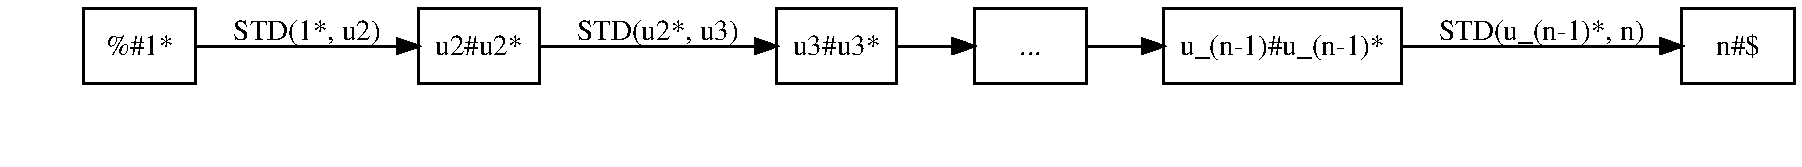
\includegraphics[width=0.9\textwidth]{pict1}
  \caption{Строка, построенная по циклу(Здесь $v*$ обозначает $\overline{v}$)}
  \label{fig:myGraph}
\end{center}
\end{figure}

Надстрока имеет длину $\sum\limits_{i = 1}^{n - 1} (2OUT(i) + 2) + (n - 2) + 4 = 2m + 3n$.
\par
Чтобы доказать обратное утверждение, мы покажем, что $2m + 3n$ это нижняя граница размера надстроки $S$ и затем покажем, что эта нижняя граница может быть достигнута только в случае если надстрока
кодирует Гамильтонов путь. Всего мы имеем $2m + n$ строк, в сумме их длина $3(2m + n)$. Наибольшее "сжатие" дает порядок, в котором каждая строка кроме первой имеет перекрытие длины 2 с обеих сторон.
Этот порядок должен дать надстроку длины $3(2m + n) - 2(2m + n - 1) = 2m + n + 2$. Однако, n - 2 коннектора могут иметь перекрытие только длины 1 с обеих сторон,
т.к. ни одна строка не начинается и не заканчивается с символа $\#$.
К тому же терминальные строки могут перекрываться максимум на 1 символ только с одной строны. Соблюдая эти условия, мы имеем нижнюю границу на длину надстроки в
$(2m + n + 2) + 2(n - 2) + 2 = 2m + 3n$ для S. Отметим, что она начинается с $\%\#\overline{1}$ и заканчивается $n\#\$$.
\par Рассмотрим два вхождения $\#$ в такую надстроку. Обозначим за $x$ то, что находится между этими двумя знаками $\#$. Первый символ из $x$ должен быть запрещенным, а
последний не запрещенным, поскольку они являются подстрокой соединителя. Если в $x$ нет соеденителей, то тогда все подстроки кроме первой и последней должны иметь перекрытие 2 с обеих сторон.
Первая строка должна быть $\overline{v}u_j\overline{v}$, следующая $u_j\overline{v}u_{j \oplus 1}$ и так далее. Более того, все строки в $A_v$ кроме двух последних должны иметь перекрытие длины 2
с обеих сторон, так каждая последующая строка должна быть "добита" уникальной строкой, которая перекрывается с ней на 2 символа. Таким образом все строки в $A_v$ должны появляться в
конкретном порядке, и если $x$ содержит одну строку из $A_v$, то он обязан содержать их все. Таким образом, $x$ - это стандартная надстрока для $A_v$
Применяя рассуждения выше ко всем вхождениям пар $\#$ мы получаем $n - 1$ различную стандартную строку. Мы можем восстановить Гамильтонов путь смотря на символы следующие за каждым вхождением $\#$,
причем запрещенные и не запрещенные символы каждого соединителя отвечают одной и той же верщине в $G$. Отметим, что в силу расположения $\%\#\overline{1}$ и $b\#\$$, мы получаем путь из $1$ в $n$
\begin{center}
  \Large
  \textbf{Построение приближенного алгоритма и доказательство 4-приблеженности}
  \normalsize
\end{center}
\defin Префиксным графом для мнжества строк $S$ назовем полный ориентированный граф, в котором вершинами являются строки из $S$, где ребро $(s_i, s_j)$ имеет вес $pr(s_i, s_j)$
\defin Обозначим за $\langle s_{i_1}, s_{i_2} ... s_{i_n} \rangle$ строку:\\
\begin{center}
 $pr(s_{i_1}, s_{i_2})pr(s_{i_2}, s_{i_3}) ... pr(s_{i_{n - 1}}, s_{i_n}) s_{i_n}$ \\
\end{center}
Пусть $S$ это множество строк из задачи о минимальной надстроке. Мы попытаемся построить другое множество $R$, такое что:\\
1) Строки в $R$ не сильно перекрываются,\\
2) Каждая строка $s \in S$ имеет надстроку в $R$, так что любая надстрока для $R$ является надстрокой для $S$,\\
3) Оптимальное решение $OPT_R$ для $R$ не сильно хуже оптимального решения $OPT_S$ для $S$.\\
Как только мы построили такое $R$ мы можем найти приближенное решение для $R$ сведением к асимметричному наибольшем пути в TSP\\
Построим множество для $R$.\\
1) Найдем минимальное покрытие циклами $\mathcal{C}$ в графе префиксов.\\
2) Для каждого цикла $C \in \mathcal{C}$, построим представление $r(C)$ содержащее все строки для $C$ как подстроки.
Пусть $C = \{s_{i_1}, ..., s_{i_k}\}$ мы можем взять $r(C) = \langle s_{i_1}, ..., s_{i_k} \rangle$\\
3) $R$ это множество всех представлений.\\


\lem Суммарная длина $\omega(\mathcal{C})$ всех циклов минимального покрытия $\mathcal{C}$ ограничена сверху величиной $\le OPT$ оптимального решения.\\
\textit{Доказательсво} Верно поскольку суммарная длина минимального покрытия циклами графа префиксов не больше чем
длина минимального $TSP$ пути графе, которая является оценкой снизу для $OPT$. (Поскольку OPT имеет вид  $\langle s_{i_1}, ..., s_{i_n} \rangle$
 и его длина больше чем цикл на этих же вершинах в префиксном графе)

\lem $OPT_R \le 2OPT_S$\\
\textit{Доказательство:}\\
Вспомним, что все строки $r \in R$ имеют вид $r = \langle  s_{i_1}, ..., s_{i_k} \rangle$. Рассмотрим немного более длинные
$\hat{r} = \langle s_{i_1}, ..., s_{i_k}, s_{i_1} \rangle$. Мы покажем, что $OPT_{\hat{R}} \le 2 OPT_S$\\
Каждая строка $\hat{r} \in \hat{R}$ начинается и кончается с одной и той же строки, обозначим ее за $s(\hat{r})$. Пусть $S(\hat{R})$ это
набор таких строк $s(\hat{r})$. Очевидно $OPT_{S(\hat{R})} \le OPT(S)$. Но отметим, что отимальное решение для $S(\hat{R})$ может быть найдено
из решения для $\hat{R}$. Просто заменим каждую $s(\hat{r})$ на соответствующуу строку $r$. Замена $s(r)$ на $r$ увеличивает длину решения
на длину цила $C$ соответствующего $r$, таким образом все замены суммарно увеличивают размер решения на $\omega(\mathcal{C})$, который оценивается
сверху по предыдущей лемме $\le OPT$.

\lem Пусть $c_1, c_2$ это два цикла минимального покрытия $C$ для графа префиксов  и пусть $r(c_1)$ и $r(c_2)$
это представления для этих циклов, как определено выше. Тогда
\begin{center}
$ov(r(c_1), r(c_2)) < \omega(c_1) + \omega(c_2)$
\end{center}
Перед тем как доказать эту лемму нам нужно сделать несколько технических определений и наблюдений.
Для любого цикла $c = s_{i_1}, ..., s_{i_k} \in \mathcal{C}$ в префиксном графе $S$, введем следующее обозначение:

\begin{center}
$s(c) = pr(s_{i_1}, s_{i_2})pr(s_{i_2}, s_{i_3})...pr(s_{i_{k - 1}}, s_{i_k})pr(s_{i_k}, s_{i_1})$
\end{center}
Обозначим за $s^{\infty}$ строку вида $ssss...$
\lem Для любого цикла $c = s_{i_1}, ..., s_{i_k}$ в префиксом графе для $S$, каждая $s_{i_j}$ является подстрокой
$\lbrack s(c)\rbrack^{\infty}$. Также, $r(c) = \langle s_{i_1}, ..., s_{i_k} \rangle$ является подстрокой $\lbrack s(c)\rbrack^{\infty}$\\
\textit{Доказательство}\\
Вспомним, что для любых $s, t$ мы имеем $s = pr(s, t)ov(s, t)$, поэтому $s$ является подстрокой (префиксом) $pr(s, t)t$
Таким образом $s_{i_j}$это префикс для строки $pr(s_{i_j}, s_{i_{j+1}})s_{i_{j + 1}}$, которая в свою очередь является префиксом для
$pr(s_{i_j}, s_{i_{j + 1}})pr(s_{i_{j + 1}, s_{i_{j + 1}}})s_{i_{j + 2}}$ и так далее. Продолжая таким же образом по циклу $c$ мы доказываем
утверждение для $s_{i_j}$. По тем же причинам доказательство работает для $r(c)$
Обратное утверждение также верно
\lem Если все строки $\hat{S} \subseteq S$ являются подстроками $t^\infty$, тогда сущетвует цикл длины $|t|$ в графе префиксов для $S$,
такой что он содержит все этим строки.\\
\textit{Доказательство.}\\
Если строка $s$ является подстрокой $t^\infty$, то она появляется в $t^\infty$ каждые $|t|$ символов. Таким образом задается циклический порядок
на строках из $\hat{S}$ и легко видеть, что этот порядок дает цикл длины $|t|$ в префиксном графе.\\
\textit{продолжение доказательства леммы 3}\\
Пусть $x, |x| \ge \omega(c_1) + \omega(c_2)$ это перекрытие $r(c_1)$ и $r(c_2)$. Тогда $x$ является подстрокой $\lbrack s(c_1) \rbrack^\infty$
(поскольку $r(c_1)$ является) и $\lbrack s(c_2) \rbrack^\infty$ (поскольку $r(c_2)$ является).
Пусть $x_1$ это префикс $x$ длины $\omega(c_1)$ и $x_2$ это префикс $x$ длины $\omega(c_2)$. Очевино, $x$ это префикс $x_1^\infty$ и $x_2^\infty.$
Теперь, поскольку $|x| \ge \omega(c_1) + \omega(c_2) = |x_1| + |x_2|$, мы имеем $x_1 x_2 = x_2 x_1$. Но это значит, что $x_1^k x_2^k = x_2^k x_1^k$
для любого $k$ (по индукции), поэтому $x_1^\infty = x_2^\infty$
\par
Любая строка в $c_1$ является подстрокой $x_1^\infty$(по лемме 4, поскольку $x_1$ является циклическим сдвигом $s(c_1)$), по этому она также является
подстрокой $x_2^\infty$. Также любая подстрока в $c_2$ является подстрокой $x_2^\infty$. Таким образом по лемме 2, все строки в циклах $c_1$ и $c_2$
сожержатся в одном цикле длины $\omega(c_2)$, что противоречит предположению, что $c_1$ и $c_2$ являются минимальными циклическими покрытиями.
\\
Из леммы 3 и леммы 1 вытекается следущее

\lem Суммарное перекрытие любого решения для множества представлений $R$ $\le 2OPT_S$\\

4-приблеженный алгоритм для имплементации:\\
1) Для множества строк $S$ построиммножество представлений $R$\\
2) Вернем конкатенацию всех строк из $R$\\
\thm
Описанный выше алгоритм является 4-приближенным алгоритмом \\
\textit{Доказательство.} Рассмотрим оптимальное решение для множества R. Длина $OPT_R$ решения $\le 2OPT_S$.
Также суммарное перекрытие этого оптимального решения $\le 2OPT_S$ по лемме 5. Но общая длина $|R|$ строк в $R$
в точности равняется сумме длин $OPT_R$ оптимального решения и его суммарного перекрытия, поэтому $|R| \le 4OPT_S$
\\
\begin{center}
\Large
\textbf{4 приближенный алгоритм}
\normalsize
\end{center}
\par

Построим граф $G = (V, E)$, где $V = 1..n, E = \{(i, j, overlap(s_i, s_j))| i, j = 1..n, i \ne j\}$ - последнее множество,
это множество троек (начальная вершина, конечная вершина, вес). Затем для данного графа $G$ найдем покрытие циклами минимального суммарного веса.
Это и будет 4-приближенный алгоритм для задачи.

% \begin{figure}[htp]
%   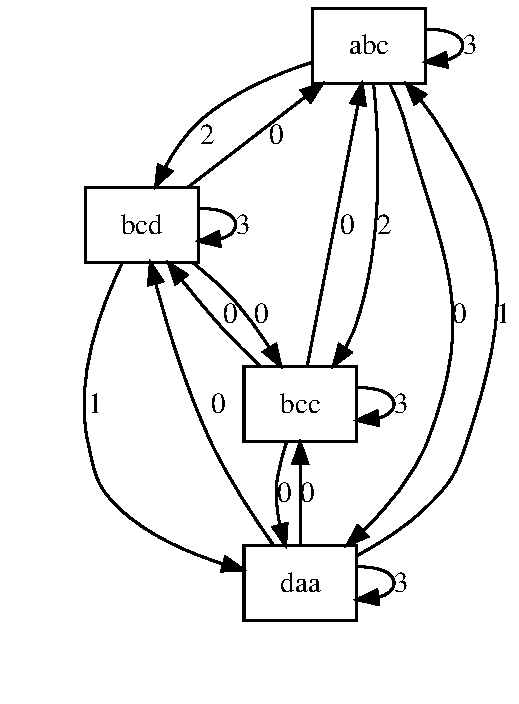
\includegraphics[scale=0.4\textwidth]{pict2}
%   \caption{Строка, построенная по циклу(Здесь $v*$ обозначает $\overline{v}$)}
%   \label{fig:myGraph}
% \end{figure}
\begin{center}
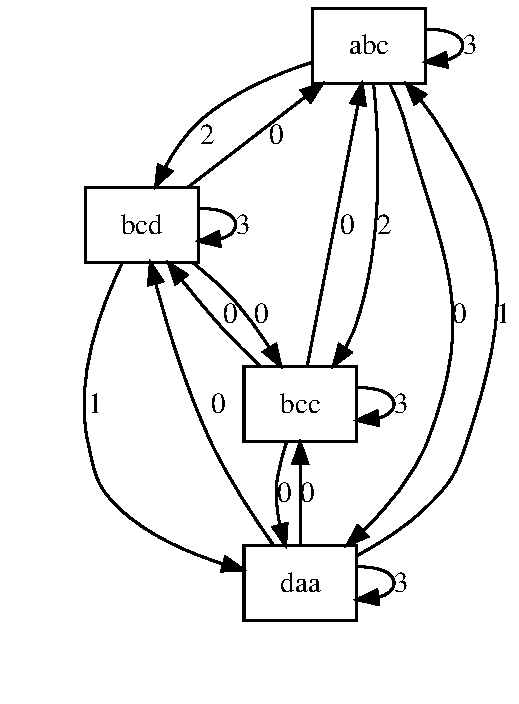
\includegraphics[width=1.6in]{pict2.eps}\\
Пример: граф построенный для ['abc', 'bcd', 'daa', 'bcc']
\end{center}
\par
\textit{Вычислим жадное назначение для данного графа $G$}
\\
Будем хранить его в массиве из n чисел, обозначим его за $A$.
\\
объявим все ребра незачеркнутыми\\
повторять пока остаются незачеркнутые ребра.\\
1)Выберем ребро (i, j) максимального веса среди незачеркнутых\\
2)Зачеркнем все рабра выходящие из i и входящие в j\\
3)A[i] = j
\par
\textit{Наконец найдем покрытие минимального суммарного веса}\\
0)Повторям пока есть непосещенные вершины.
\\
1) Возьмем вершину непосещенную вершину $i$. Отметим как посещенную. Положим $s = i$\\
2)while True:\\
Далее если $A[i]$ совпадает с $s$, то добавим цикл в результат, закончить цикл, перейти к пункту $(0)$\\
иначе $i = A[i]$
\begin{center}
\Large
\textbf{Запуски описанного алгоритма, проверка 2-приближенности жадного алгоритма для маленьких строк}
\normalsize
\end{center}
Далее приведен Ipython notebook. К сожалению nbpdfconverter не поддерживает кириллицу, поэтому пояснения приведены на английском.

\setboolean{@twoside}{false}
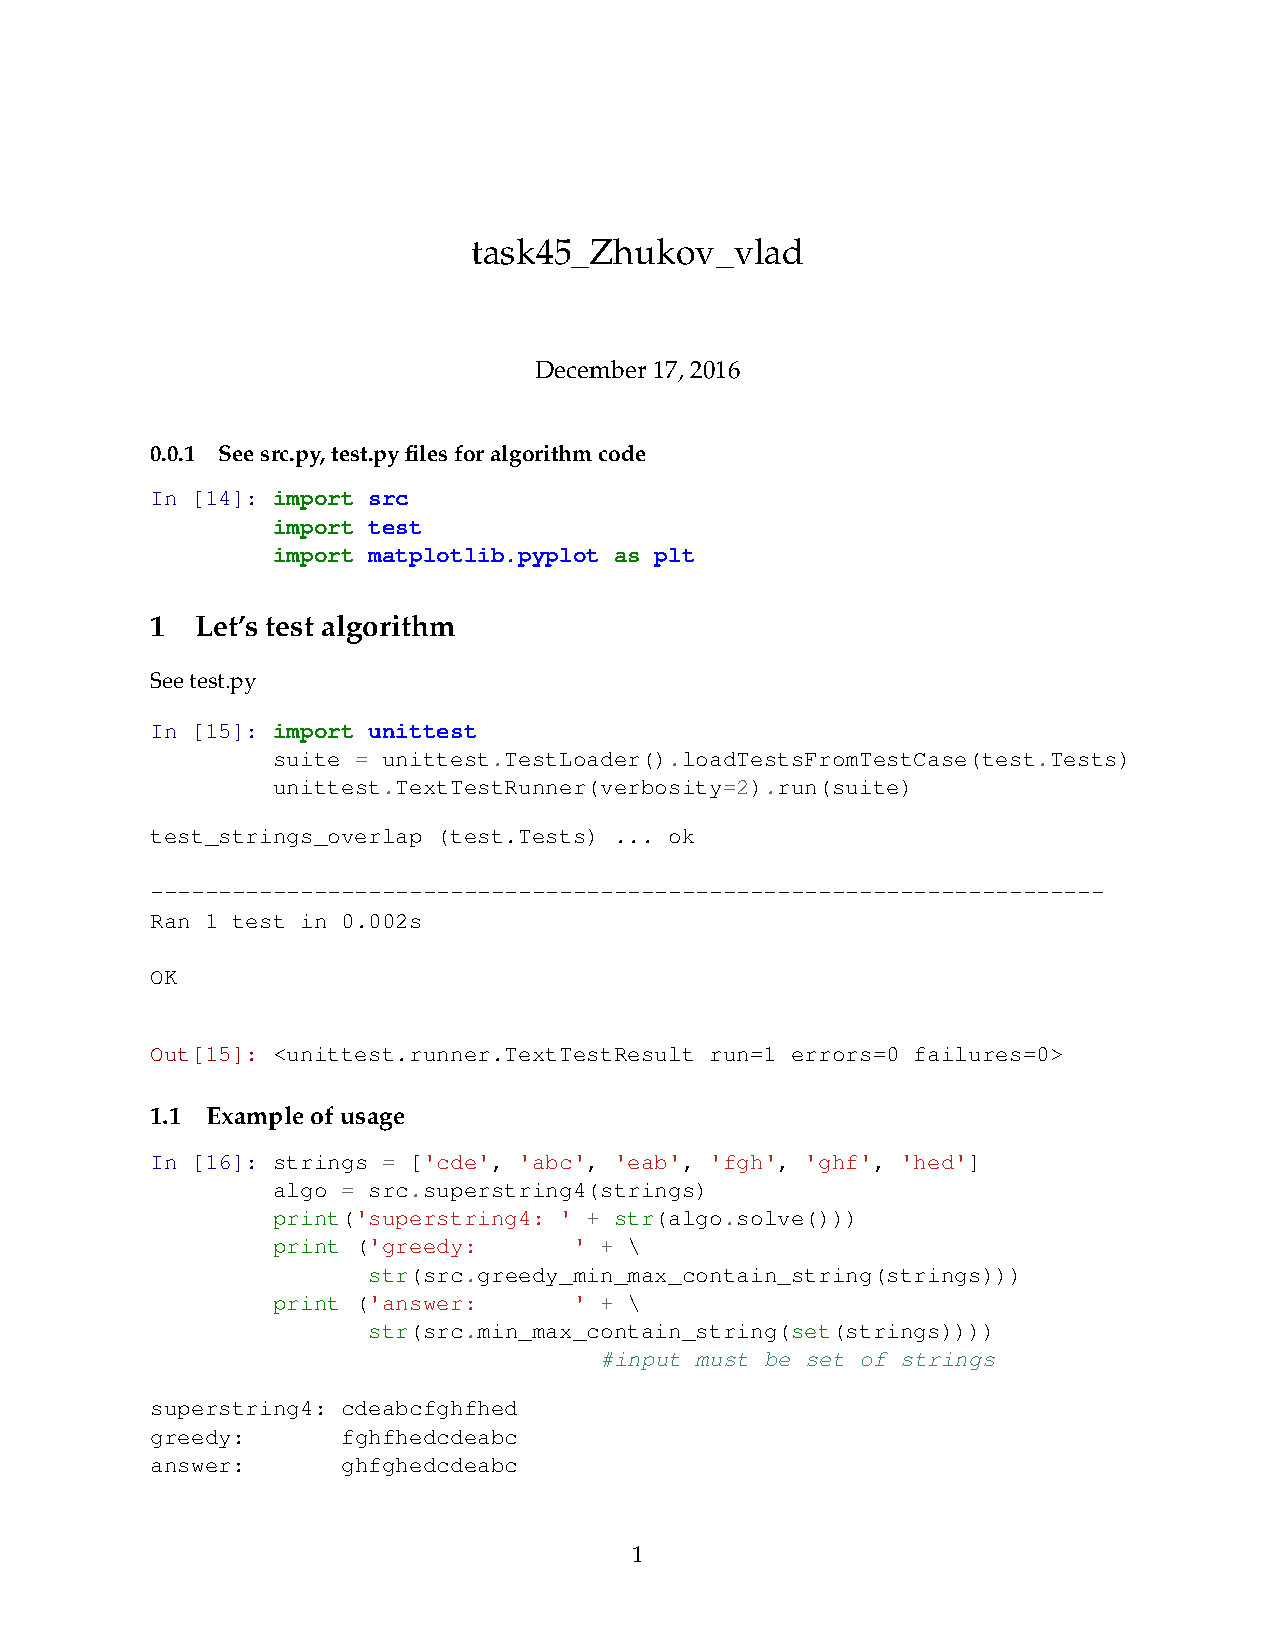
\includepdf[pages=-, offset=15 -75]{notebook.pdf}
\begin{center}
\Large
\textbf{Имплементация алгоритмов. src.py}
\normalsize
\end{center}
\par
\lstset{
  caption=,
  basicstyle=\footnotesize, frame=tb,
  xleftmargin=-.0\textwidth, xrightmargin=.2\textwidth
}
\lstinputlisting[language=Python]{src.py}
\begin{center}
\Large
\textbf{test.py}
\normalsize
\end{center}
\lstinputlisting[language=Python]{test.py}

\begin{thebibliography}{9}
\bibitem{lamport94}
 J Gallant, D Maier, J Astorer
  \emph{ On finding minimal length superstrings},
  Journal of Computer and System Sciences, 1980 - Elsevier
\bibitem{lamport94}
  Jonathan S. Turner
  \emph{ APPROXIMATION ALGORITHMS FOR THE SHORTEST COMMON SUPERSTRING PROBLEM},
  Computer Science Department Washington University, St. Louis
\bibitem{lamport94}
Marcin Mucha
  \emph{A Tutorial on Shortest Superstring Approximation}
  December 17, 2007
\end{thebibliography}
\end{document}
